\documentclass[paper-main.tex]{subfiles}

\begin{document}

The basic physics of gravitational-wave detection can be demonstrated with a table-top Michelson interferometer, an optical configuration commonly used in undergraduate labs. 
A simple Michelson interferometer comprises a laser, a beamsplitter, and two mirrors. 
Laser light is split by a beamsplitter into two arms at right angles. 
At the end of each arm is a mirror which reflects the beams back to the beamsplitter where they recombine. 
The combination of the two beams produces an interference pattern which is dependent on the relative distance travelled by each of the beams. 
A change in arm length results in a change in the interference pattern. 



Gravitational-wave detectors are large, complex interferometers.
The LIGO and Virgo detectors have $4\,{\rm km}$ and $3\,{\rm km}$ arms respectively.
They are sensitive to minuscule changes in distance, for example the first detection of a binary black hole merger had a peak gravitational-wave strain of $10^{-21}$ ~\cite{GW150914}.
However, their design is based fundamentally on the Michelson interferometer. 
Detection and analysis concepts can be demonstrated with table-top optical equipment. 
 



A commonly-used analogy in explaining gravitational-wave science is sound. 
Signals of binary black hole and neutron star mergers can be converted into audio as an aid to explanations~\cite{SoundsOfSpaceTime:online,BlackHoleHunter:online}~\footnote{When introducing the acoustic analogy to lay audiences, it ins important to emphasize that gravitational waves are not sound. For example, gravitational waves can propagate in a vacuum, whereas sound cannot.}.
Sound vibrations provide a simple means to move the components of a demonstration interferometer. 
The vibrations move the mirrors, changing the length of the interferometer arms, and the resulting interference pattern. 
We use sound throughout this work as a means of simulating gravitational-wave-like signals and the data analysis and signal processing techniques used to detect them.



\begin{figure}
% 	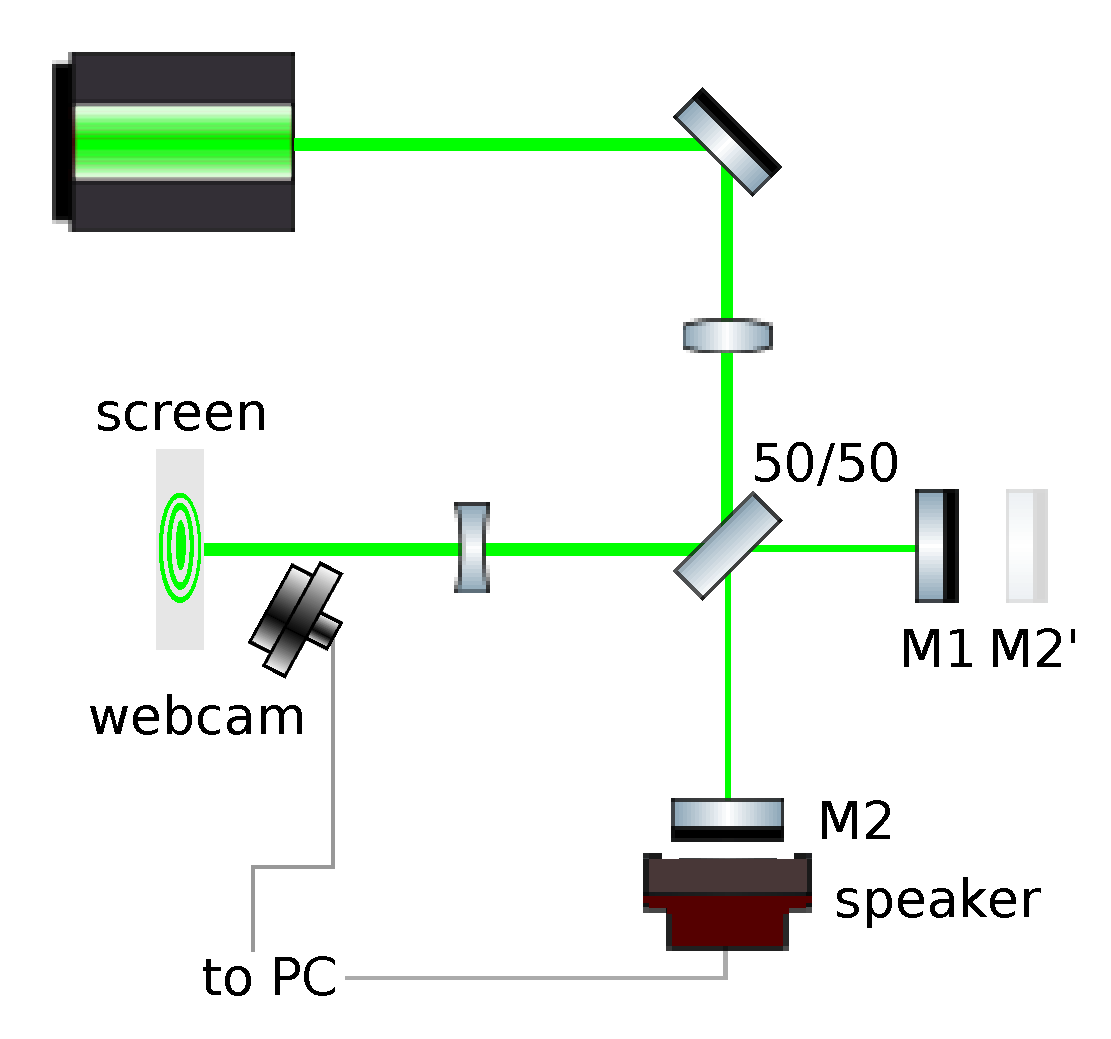
\includegraphics[width=0.49\textwidth]{figures/ifo_schematic_webcam.pdf}
	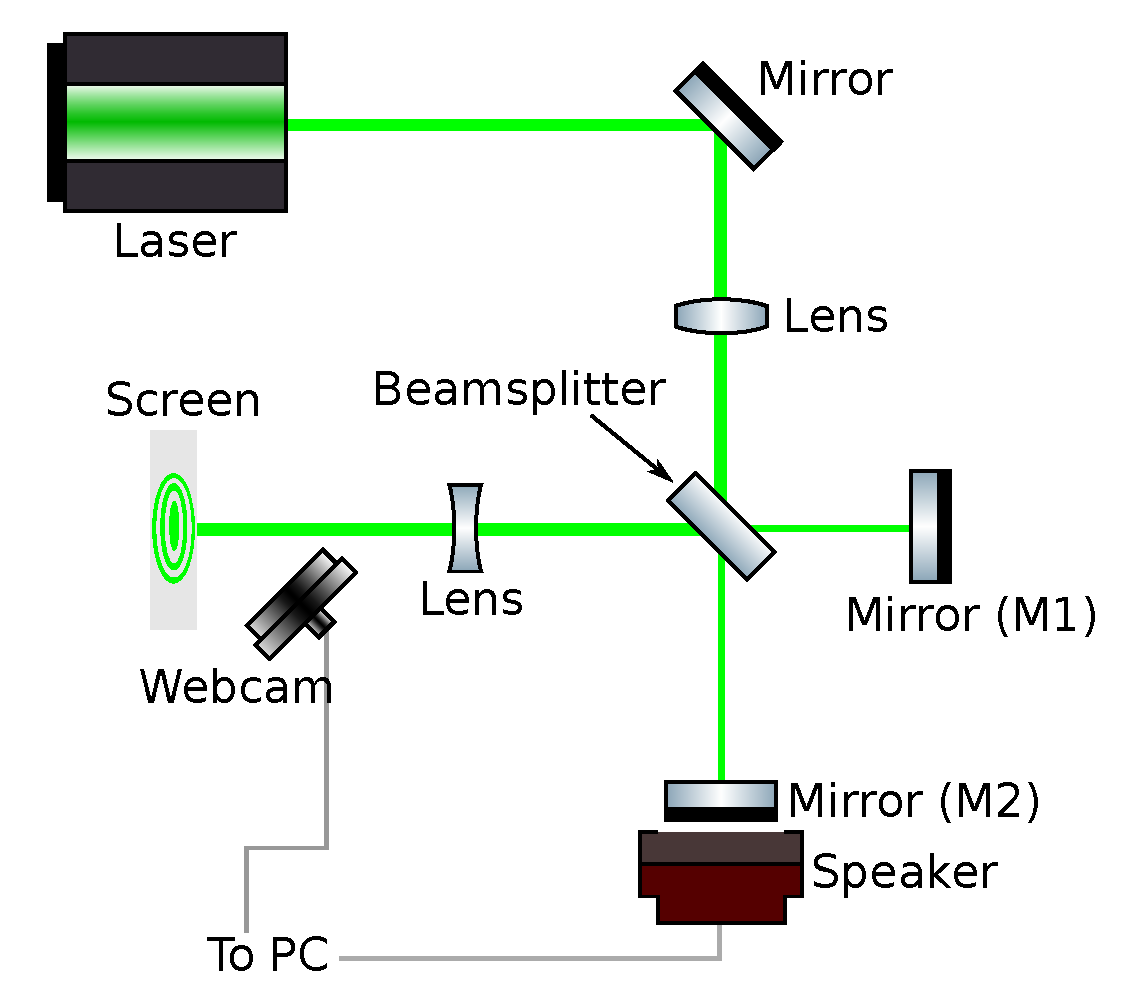
\includegraphics[width=0.49\textwidth]{figures/ifo_schematic_webcam_edit.pdf}
	\caption{\label{fig:ifo_schematic_webcam}
Schematic of the table-top Michelson interferometer. 
The laser (top-left) is a Class 2 $532\,{\rm nm}$ laser~\cite{ThorLabsIFO}. 
The beam is first reflected from a mirror at a right angle and then focused at a converging lens before the beamsplitter which is $50$/$50$ in reflection and transmission. 
The split beams are reflected from mirrors (M1 and M2) at the ends of the interferometer arms and are recombined at the beamsplitter. 
The beam is enlarged by a diverging lens after the beamsplitter. 
The interference pattern is projected onto a screen and recorded using a commercial webcam connected to a personal computer (PC). 
A speaker fixed to the back of M2 provides the signal input from the PC.  
%Michelson interferometer schematic with interference pattern recorded by a commercial webcam. The laser (top-left) is a Class 2 $532\,{\rm nm}$ laser~\cite{ThorLabsIFO}. The beam is first reflected from a mirror a right angle (to save space on the optical breadboard) and then focused at a converging lens before the $50$/$50$ beamsplitter. The split beam is reflected from mirrors M1 and M2 at the ends of the interferometer arms and recombined at the beamsplitter. The interference pattern is enlarged by a diverging lens after the beamsplitter and projected onto a screen. A commertial speaker is fixed to the back of M2, as the signal input. The interferometer arms lengths are roughly $3\,{\rm cm}$ different and the entire interferometer (without the screen) fits within the dimensions of an A4 piece of paper. We did not include a compensating plate with the beamsplitter, as is often done.} 
    }
\end{figure}

The Michelson interferometer configuration used in this work is shown schematically in Fig.~\ref{fig:ifo_schematic_webcam}.
It is constructed on a $450 \times 450 \,{\rm mm} $ optical breadboard. 
The laser (top-left) has a wavelength of $532\,{\rm nm}$.
In the configuration shown in Fig.~\ref{fig:ifo_schematic_webcam} the laser beam is first reflected from a mirror which turns the beam $90^{\circ}$ (to save space on the optical breadboard). 
The beam passes through a converging lens and then to the beamsplitter, which is $50$/$50$ reflection and transmission. 
The beams are reflected by mirrors at the end of each of the two arms ($\approx 7.5\,{\rm cm}$ and $\approx 10.0\,{\rm cm}$ long) and are recombined at the beamsplitter. 
The resulting interference pattern is projected onto a screen and recorded by a webcam. 


The interference pattern is a ring of interference fringes as shown by the photograph in Fig.~\ref{fig:interference_pattern}. 
The pattern is enlarged by a diverging lens between the beamsplitter and the screen to aid in viewing. 
A change in the relative length of the interferometer arms results in the interference rings moving radially inwards or outwards. 
Ring interference patterns like this are often used in gravitational-wave table-top demonstrations to allow changes in the pattern to be easily viewed. 
%This results in a phase difference between the two beams when they meet at the screen. This path difference is perhaps better seen as the perpendicular separation between one mirror (M1) and the virtual image (M2\textquotesingle) of the other. For an aligned configuration and a fixed separation, the phase difference at a point on the screen only depends on the angle from the centre-line of the beam, and so the pattern is circularly symmetric. When the path difference changes, the fringes stay circular but move radially in or out.
%A ring interference pattern is often used in gravitational-wave table-top demonstrations to allow changes in the pattern to be easily seen. 


\begin{figure}
 \begin{center}
  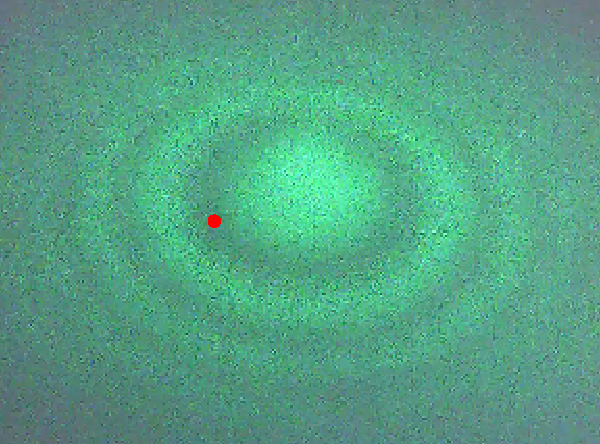
\includegraphics[width=.45\textwidth]{figures/webcam_still0_crop.pdf}
 \end{center}
 \caption{\label{fig:interference_pattern}
Michelson interference pattern as viewed by an off-axis webcam (which is why the pattern is elliptical). 
The red dot marks where the intensity time series is measured. 
The central bright fringe of the interference pattern is approximately $5\,{\rm mm}$ in diameter. 
% Interference pattern from Michelson interferometer as viewed by webcam from off-centre (hence why the pattern appears non-circular), red dot indicates point where intensity time series was measured from. For scale, the central fringe is approximately $5\,{\rm mm}$ across.
}
\end{figure}


A $0.5\,{\rm W}$ speaker is fixed to the back of one of the mirrors (M2 in Fig.~\ref{fig:ifo_schematic_webcam}), providing a controllable source of vibrations. 
The speaker is one half of a pair of commercial, USB-powered speakers fed by a $3.5\,{\rm mm}$ jack and driven by a PC. 
It is attached to the back of the mirror using commercial adhesive putty. 
The other speaker in the pair is kept face-down and as far away from the interferometer as the cables to reduce its impact as a second source of vibrations. 


%As the speaker deforms to play sound, the mirror moves producing a change in arm length related to some coupling function of the amplitude and frequency of the audio. 
The motion of the interference fringes follows the motion of the mirror, and therefore the speaker. 
If the fringe motion is small, then changes in the intensity at some point on the screen occur at the same frequency as the injected audio but with amplitude given by a transfer function that accounts for the coupling and resonance of the speaker-mirror system.
If the fringe motion is large enough for multiple fringes to pass over the measured point in a single speaker deformation, then over-counting artificially raises the measured frequency. As such, any motion of the fringes must be kept small by playing sound softly through the speaker.
Even without over-counting, large fringe motions introduce a nonlinear relation between the intensity fluctuations and injected audio, leading to troublesome - but physically interesting! - phenomena like frequency doubling.
We derive the non-linear relation between the separation of the mirrors and the intensity of the pattern at some point on the screen in Appendix~\ref{app:intensity_derivation}. 


Data can be recorded via a webcam (as shown in Fig.~\ref{fig:ifo_schematic_webcam}) or photo-diode. 
In Sections~\ref{sec:single_tone} and~\ref{sec:viterbi_wandering} a webcam is used. 
In Section~\ref{sec:optical_microphone}, which considers more complex audio, we turn to a photodiode because it offers a higher sample rate than the webcam. 


\han{to do: add some text referring to other demo designs and references:~\cite{TTExhibit:2020,TTExhibit:online,ThorLabsIFO,LIGOIFOGlue,LIGOIFOMagnets,FoxEtAl:1999}. }
% Note that we do not include the common compensating plate that equalises the amount of time spent in glass for each beam. We did not find it necessary to include it to be able to demonstrate the results desired.







\begin{comment}
Even though gravitational waves are caused by some of the most massive events in the universe, their observable effects on Earth are vanishingly small | on the order of only one part in $10^{21}$ for our best detectors~\cite{GW150914}. Clearly, the measurement of such effects is far beyond any table-top experiment. But, the fundamental principle of gravitational wave detection remains that changes in the lengths of the beam arms of an interferometer leads to a change in the interference pattern observed. By observing sound waves that vibrate the mirrors of a table-top interferometer and so change the lengths of the beam arms we have an analogue of this principle.


\subsection{Method of Michelson interferometry to observe sound}
% hardware: path difference, virtual thin film interference

In a Michelson interferometer, a coherent (monochromatic and equal phase) source of laser light is split evenly by a beamsplitter into two arms at right-angles to each other, travelling down and back from a mirror at the end of each arm. The beams recombine and interfere at the beamsplitter before hitting a screen to produce a pattern of concentric, circular fringes. The configuration used in this experiment is shown diagrammatically in Figure~\ref{fig:ifo_schematic_webcam} and as part of a photo in Figure~\ref{fig:setup_pic2}.


A sample interference pattern is shown in Figure~\ref{fig:interference_pattern}.
This pattern is due to the path difference between the two arms of unequal lengths (if the lengths were equal, then only a single, bright dot would be seen). This results in a phase difference between the two beams when they meet at the screen. This path difference is perhaps better seen as the perpendicular separation between one mirror (M1) and the virtual image (M2\textquotesingle) of the other. For an aligned configuration and a fixed separation, the phase difference at a point on the screen only depends on the angle from the centre-line of the beam, and so the pattern is circularly symmetric. When the path difference changes, the fringes stay circular but move radially in or out.



We used a 0.5W speaker stuck to the back of one of the mirrors as an audio source for our demonstration. This speaker was part of a commercial 3.5mm-jack, USB powered pair of speakers and was driven by a PC. To attach the speaker to one of the mirrors, we wedged it into part of the mirror mount and used commercial adhesive putty to keep it in place. We kept the other speaker in the pair face-down and as far away from the experiment as the cables would allow to reduce it acting as a second source.

As the speaker deforms to play sound, the mirror moves with a change in separation as some coupling function of the amplitude and frequency of the sound. The motion of the fringes follows this motion of the mirror and therefore the speaker at the same frequency.
If the fringe motion is small, then changes in the intensity at some point on the screen follow the frequency of the injected audio but with amplitude given by a transfer function that accounts for the coupling and resonance of the speaker-mirror system.
If the fringe motion was large enough for multiple fringes to pass over the measured point in a single speaker deformation, then over-counting would artificially raise the measured frequency. As such, any motion of the fringes must be kept small by playing sound softly through the speaker.

For later sections, we derive the non-linear relation between the separation of the mirrors and the intensity of the pattern at some point on the screen, this can be found in Appendix~\ref{app:intensity_derivation}.

% Note that we do not include the common compensating plate that equalises the amount of time spent in glass for each beam. We did not find it necessary to include it to be able to demonstrate the results desired.

\begin{figure}[h]
	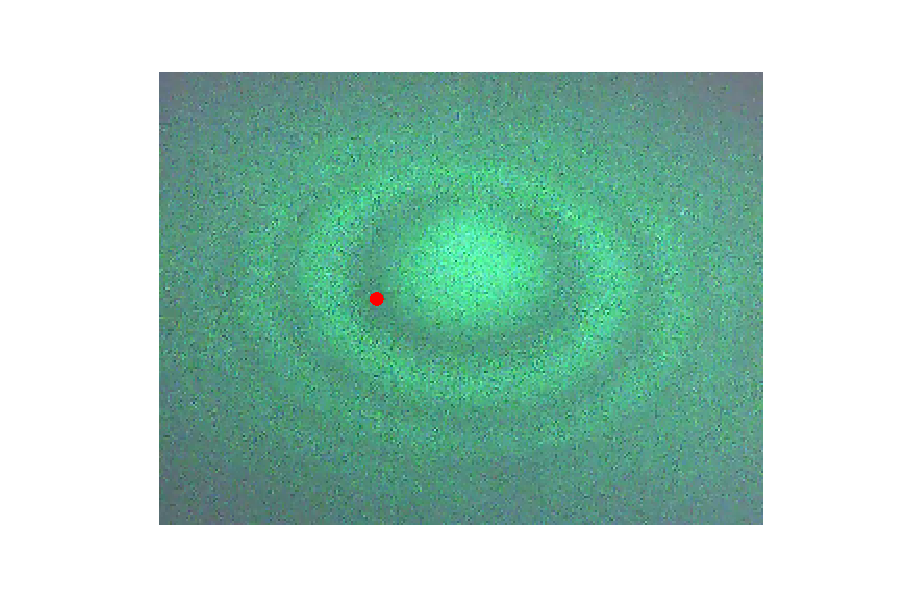
\includegraphics[width=\textwidth]{figures/webcam_still0.pdf}
	\caption{Interference pattern from Michelson interferometer as viewed by webcam from off-centre (hence why the pattern appears non-circular), red dot indicates point where intensity time series was measured from. For scale, the central fringe is approximately 5mm across}
	\label{fig:interference_pattern}
\end{figure}
\end{comment}

\end{document}
